
\documentclass[
12pt,
a4paper,
pdftex,
czech,
titlepage
]{report}

\usepackage{float}
\usepackage[czech]{babel}
\usepackage[utf8]{inputenc}
\usepackage{lmodern}
\usepackage{textcomp}
\usepackage[T1]{fontenc}
\usepackage{amsfonts}
\usepackage{titlesec}
\usepackage{graphicx}
\usepackage{longtable}
\usepackage{multirow}
\usepackage{tabularx} 
\usepackage[unicode]{hyperref}
\usepackage{indentfirst}
\hypersetup{
    colorlinks=true,
    citecolor=green,
    filecolor=black,
    linkcolor=black,
    urlcolor=magenta
}
\titleformat{\chapter}
  {\normalfont\LARGE\bfseries}{\thechapter}{1em}{}
\titlespacing*{\chapter}{0pt}{0ex plus 1ex minus .2ex}{2.0ex plus .2ex}



\begin{document}

\begin{titlepage}
	\vspace*{-2cm}
	{\centering
\includegraphics[scale=1.5]{FAV_logo.pdf}\par}
	\centering
	\vspace*{2cm}
	{\Large Dokumentace k semestrální práci z KIV/PIA\par}
	\vspace{1.0cm}
	{\Huge\bfseries KIVBOOK\par}
	\vspace{7cm}

	\begin{flushleft} 
	\begin{table}[ht]
	\label{stats}
	\begin{tabular}{ll}
	\textbf{Student:}  & Martin Kružej   \\
	\textbf{St. číslo:}   & A17N0079P    \\
	\textbf{E-mail:}  & kruzej@students.zcu.cz  \\
	\textbf{Datum:}    & \today            \\ 
	\end{tabular}
	\end{table}
	\end{flushleft}
	
	\vfill


\end{titlepage}

\tableofcontents
\thispagestyle{empty}
\clearpage

\chapter{Zadání}
\setcounter{page}{1}

Standardní téma KIV/PIA, viz \href{https://courseware.zcu.cz/portal/studium/courseware/kiv/pia/samostatna-prace/standardni-tema.html}{KIV/PIA courseware}.

\chapter{Architektura aplikace}

\section{Obecná architektura}

Aplikace je postavená na technologii Java EE. Jednoduchý diagram ukazující základní obecný chod aplikace je uveden na diagramu \ref{general}. Uživatel pracuje s tzv. front-endme, který je na klientovi ve formě HTML a CSS. Při zaslání požadavku je tento požadavek předán tzv. back-endu. Zde je zpracován jedním ze servletů, ti v případě potřeby mohou volat databázi přes třídy Manažerů a Dao. Poté vyberou některý z JSP souborů dle požadavku a ten vrací zpět na front-end, kde je zobrazen již ve formátu HTML a CSS. K architektuře bude řečeno více detailů v následujících kapitolách.

\begin{figure}[H]
\caption{Obecná architektura}
\label{general}
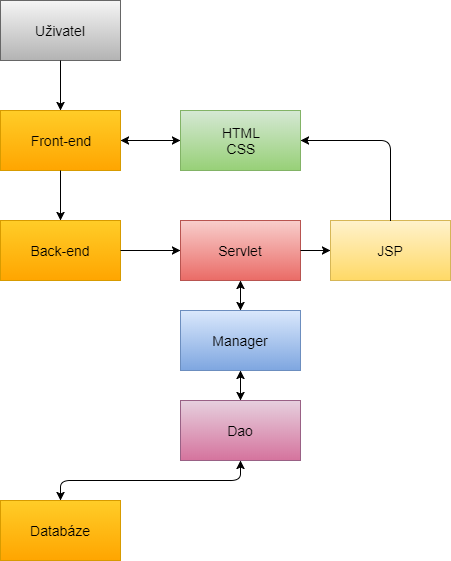
\includegraphics[width=\textwidth]{general.png}
\end{figure}

\section{Architektura servletů}

Servlety jsou základní kámen serveru - tyto servlety obsluhují veškeré požadavky, které na server chodí. Pro přístup k databázi využívají různé manažery a tyto manažery jim musí někdo poskytnout. Máme zde třídu ApplicationContext, která vytvoří všechny potřebné třídy Manažerů a Dao. Při inicializaci je spuštěn StartupListener, který třídy z ApplicationContext injekčně dopraví do servletů, které to potřebují. Tento styl se často označuje jako \textit{Dependency injection}. 

Při vyslání požadavku na server se tento požadavek nedostane k servletům hned. Nejdříve projde EncodingListener, jenž zajišťuje kódování charakterů ve formátu UTF-8. Dále jsou určité servlety za jakousi bránou, která je brání před neautorizovaným přístupem. Tato brána je AuthenticationGuard využívající AuthenticationService. Tyto dvě třídy pouze kontrolují, že pro přístup k některým servletům je třeba být přihlášen.

Diagram znázorňující tuto architekturu je uveden na obrázku \ref{servlety}.

\begin{figure}[H]
\caption{Architektura servletů}
\label{servlety}
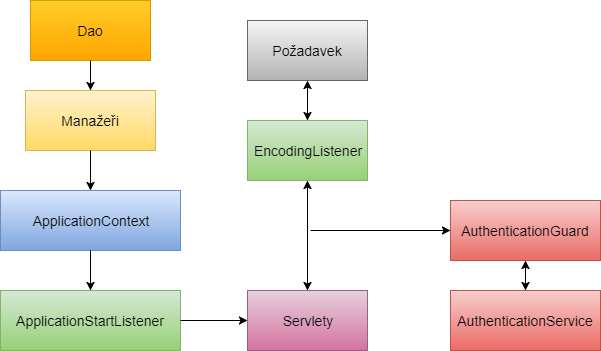
\includegraphics[width=\textwidth]{servlety.png}
\end{figure}

\section{Architektura entit}
Před podíváním o Manažerech je třeba se podívat na nejnižší úroveň této architektury a to jsou entity. Tyto entity jsou v podstatě tabulky, které se v databázi používají. Nejdříve je zde rozhraní IEntity, které dědí abstraktní třída BaseEntity. Tyto dvě třídy poskytují jednotné \textit{id} pro všechny entity. Ty existují následující:
\begin{itemize}
\item \textbf{User} - uživatel v databázi
\item \textbf{Status} - status/tweet v databázi
\item \textbf{Friendship} - přátelství / požadavek na přátelství v databázi
\end{itemize}

Následuje dědění abstraktní třídy entitami. Tento vztah je vyobrazen na obrázku \ref{entity}.

\begin{figure}[H]
\caption{Architektura entit}
\label{entity}
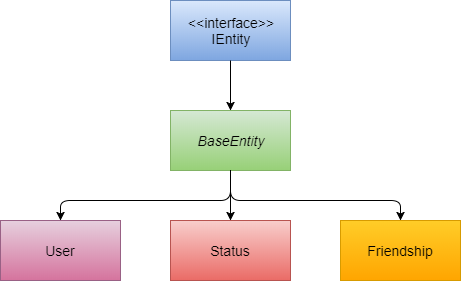
\includegraphics[width=\textwidth]{entity.png}
\end{figure}

\section{Architektura Manažerů}
Manažeři mají za úkol poskytnout prostředníka mezi servlety a databází, potažmo Dao. Poksytují různé metody pro práci s databází či entitami. Opět se zde setkáváme s rozhraními, ze kterých jsou potom odvozeny samotné třídy. Pro každou jednotlivou entitu existuje jednotliví Manažer. Servlety obecně pracují právě s rozhraním, které je jim injektováno a již je jim jedno, jakou implementaci Manažerů používají.

Vyobrazeno na obrázku \ref{manazeri}.

\begin{figure}[H]
\caption{Architektura Manažerů}
\label{manazeri}
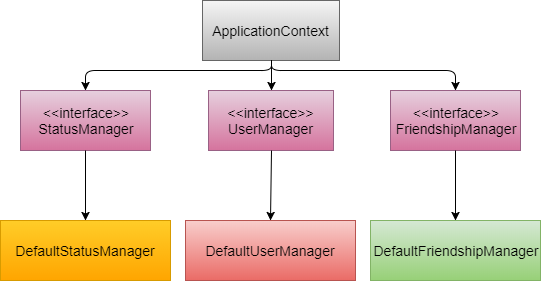
\includegraphics[width=\textwidth]{manazeri.png}
\end{figure}

\section{Architektura Dao}
Tato úroveň pracuje s databází. Přes rozhraní slibuje různé metody pro tuto práci a poté je i implementuje. Vzhledem k tomu, jak je tato architektura navržena, je možno udělat několik různých implementací těchto Dao tříd. V aplikaci je použito Criteria, ale je možno udělat třeba JPQL pouhým přidáním tříd a změnou injektování. 

Základní rozhraní je GenericDao, kde se definují ty nejzákladnější metody, které každé Dao musí implementovat - jako najít instanci, uložit instanci, smazat instanci. Toto rozhraní dědí rozhraní deklarující již specifické metody pro různé entity - FriendshipDao, UserDao a StatusDao. Tyto třídy jsou to rozhraní, které je injektováno třídou ApplicationContext.

Následuje specifikace JPA. Nejdříve obecná třída GenericDaoJpa s velice obecnými metodami. Následují abstraktní třídy pro jednotlivé entity. Tyto třídy dědí jak GenericDaoJpa tak jednotlivé Dao rozhraní. Poslední částí architektury jsou samotné implementace jednotlivých metod. Jak bylo řečeno v předešlých odstavcích, tato aplikace využívá Criteria, ale zde by mohly být další třídy, např. FriendshipDaoJPQL využívající JPQL. 

Vyobrazeno na obrázku \ref{dao}.

\begin{figure}[H]
\caption{Architektura Dao}
\label{dao}
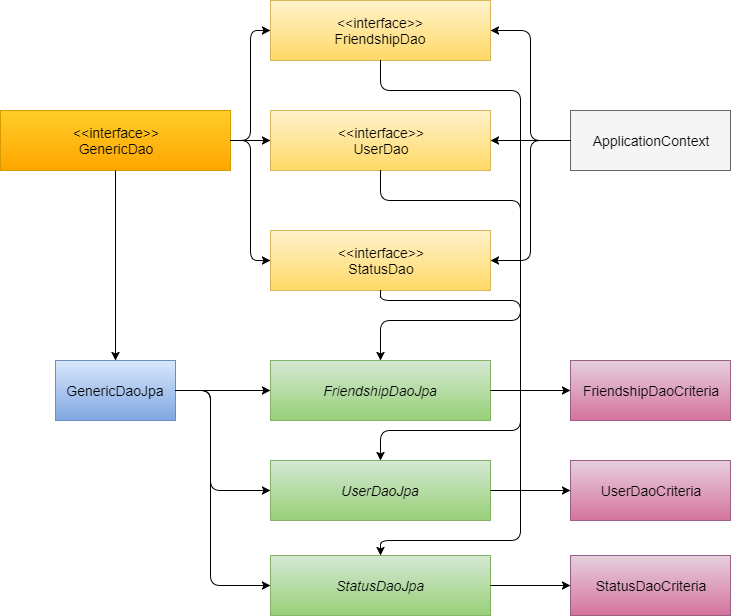
\includegraphics[width=\textwidth]{dao.png}
\end{figure}

\chapter{Aplikace}

\section{Use case}

Aplikace imituje některé známé sociální sítě. Use case aplikace je vyobrazen na obrázku \ref{use_case}.
Horní část diagramu ve světlé žluté je ta část, která je přístupná nepřihlášenému uživateli. Tento uživatel si může prohlížet některé statické stránky, seznam registrovaných uživatelů a profily těchto uživatelů. Přístup ke zbytku aplikace mu bude zamítnut dokud se nezaregistruje/nepřihlásí.

Po přihlášení do systému je uživateli zpřístupněn zbytek aplikace. Dostává nyní vlastní zeď, může upravovat svůj profil, dívat se na své přátele, žádat o přátelství, zamítat přátelství a také vytvářet statusy a lajkovat/hejtovat je. 

\begin{figure}[H]
\caption{Use case}
\label{use_case}
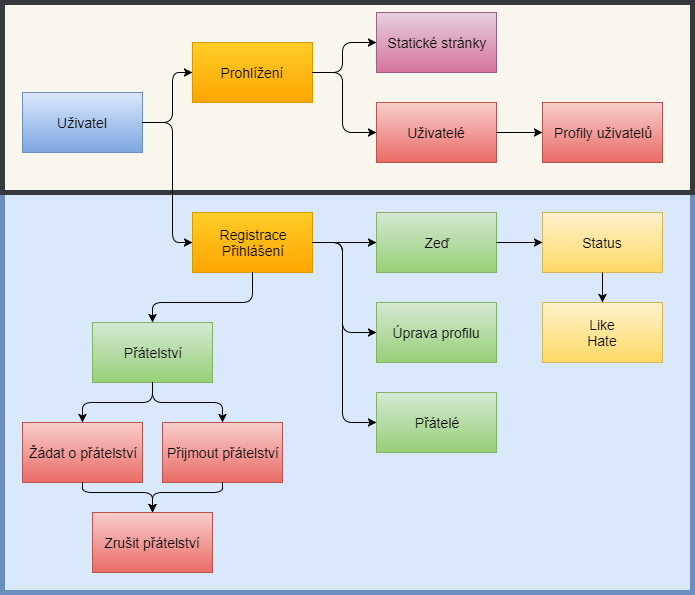
\includegraphics[width=\textwidth]{use_case.png}
\end{figure}

\section{Prohlížení stránek}

Aplikace dovoluje nepřihlášenému uživateli prohlédnout si některé stránky. Může se podívat na názory některých uživatelů či informace o aplikaci. Je mu dovoleno zhlédnout seznam registrovaných uživatelů a může si prohlížet jejich profily. Sám nikde nenajde nikdy odkaz, který by ho zavedl do privilegované části aplikace, ale chytrý uživatel může samozřejmě měnit URL. Proto je v aplikaci AuthenticationGuard, který nepřihlášeného uživatele nikam dál nepustí a vybídne ho k přihlášení.

\section{Registrace}

Uživatel má možnost se zaregistrovat. Bude mu nabídnut registrační formulář s následujícími položkami:
\begin{itemize}
\item \textbf{Uživatelské jméno} - uživatelovo jméno, kterým se bude přihlašovat - \textbf{povinné}
\item \textbf{Heslo} - heslo k uživatelskému účtu - \textbf{povinné}
\item \textbf{Kontrola hesla} - znovu zadání hesla - \textbf{povinné}
\item \textbf{Pohlaví} - jestli je uživatel muž, či žena - \textbf{nepovinné}
\item \textbf{Datum narození} - kdy se uživatel narodil - \textbf{nepovinné}
\item \textbf{Souhlas s podmínkami} - uživatel souhlasí s podmínkami - \textbf{povinné}
\item \textbf{Kontrola robotů} - uživatel je nucen napsat číslici 4 - \textbf{povinné}
\end{itemize}

Povinné položky formulář nepovolí odeslat, dokud nejsou vyplněny. Uživatelské jméno je povoleno pouze písmena a číslice. Hesla se musejí shodovat. Datum narození nemusí být vyplněn vůbec ale pokud uživatel vyplní pouze část data, je mu vynadáno. Heslo je dále hashováno, než je uloženo do databáze. V případě chybných údajů, například že se neshodují hesla, je formulář předvyplněn některými údaji, jmenovitě uživatelské jméno, pohlaví, souhlas s podmínkami a kontrola robotů.

\section{Přihlášení}

Při přihlášení uživatel vyplňuje svoje uživatelské jméno a heslo. V případě neshody je uživatel nepřihlášen. Po úspěšném přihlášení se schovávají položky pro přihlášení/registraci a jsou nahrazeny profilem a odhlášením. Nyní je uživatel volný kamkoliv do aplikace. Žádný odkaz nevede zpátky do statických stránek, ale chytrý uživatel si samozřejmě poradí. Pokud se přihlášený uživatel dostane zpět na stránky registrace a přihlášení, jednoduše mu nebude dovoleno žádnou z forem vyplňovat, dokud bude přihlášen.

\section{Prohlížení uživatelů}

Přihlášený uživatel si také může prohlédnout ostatní uživatele. Po kliknutí na jejich uživatelská jména vidí jejich profily. Může si také prohlédnout své přátele, pokud nějaké má, v záložce \textit{přátelé}. U profilů na rozdíl od nepřihlášených uživatelů vidí další tlačítka. Jde o:
\begin{itemize}
\item Pokud není s uživatelem přítel, uvidí \textit{Poslat žádost o přátelství}
\item Pokud jsou přátelé, uvidí \textit{Zrušit přátelství}
\item Pokud jeden z nich zažádal o přátelství, neuvidí nic
\end{itemize}

Detaily k přátelství budou popsány v dalších kapitolách.

\section{Úprava profilu}

Pokud se uživatel dostane k prohlížení svého profilu, nebude si prohlížet ale má možnost ho změnit. Z klasických je podpora pro: heslo, email, pohlaví. Uživatel zde má možnost také nahrát nový profilový obrázek. Stačí jej vybrat a kliknout na \textit{Nahrát}. 

\section{Přátelství}

Uživatelé mohou mezi sebou vytvářet přátelství. Jde o oboustrannou dohodu. Jeden z uživatelů musí vždy požádat o přátelství - přes profily, jak bylo řečeno. Druhý musí tuto žádost potvrdit. Všechny žádosti jsou zobrazeny na Zdi. Zde uživatel vidí odchozí žádosti, které podal a příchozí žádost, které mu ostatní posílají. U svých žádostí má možnost je stáhnout, čímž je zruší. U příchozích je buď přijme, čímž vzniká přátelství, nebo bude ignorovat, čímž se zruší.

Přátelství zajišťuje přidání uživatele do záložky \textit{Přátelé} a jeho statusy se budou zobrazovat na zdi uživatele. Přátelství se dá kdykoliv zrušit - stačí jít na profil přítele a stisknout \textit{Zrušit přátelství}. Uživatel je odebrán ze seznamu přátel a jeho statusy se již nebudou zobrazovat.

\section{Statusy}

Uživatel může vytvářet statusy. Na stránce Zeď je možnost vyplnit text statusu a poté kliknout na \textit{Statusovat}, čímž se vytvoří nový status. Automaticky je zobrazen čas, kdy byl status napsán. Tento status je viditelný pro samotného uživatele a jeho přátele.

Každý status lze lajkovat či hejtovat. Stačí kliknout na tlačítko \textit{Lajkovat} či \textit{Hejtovat}. Seznam těch, kteří určitý status lajkovali/hejtovali je umístěn pod statusem stejně jako celkový počet těchto lajků/hejtů. Uživatel může jeden status:
\begin{itemize}
\item Lajkovat
\item Hejtovate
\item Lajkovat poté, co lajkoval, tím zruší lajk
\item Hejtovat poté, co hejtoval, tím zruší hejt
\item Pokud se pokusí mixovat, tedy lajkovat poté co hejtoval, aplikace mu vynadá
\end{itemize}

Lajky a Hejty nezanikají se zánikem přátelství.

\section{Zeď}
Zeď je hlavní středisko aplikace. V pravé části jsou notifikace - příchozí a odchozí žádosti a lze s nimi manipulovat. Uprostřed je možnost psát statusy. Pod tím jsou zobrazeny statusy přátel a uživatele. Vždy se zobrazují po deseti a je možno mezi nimi procházet, pokud jich je hodně. Platí:
\begin{itemize}
\item Pokud je statusů méně než 10, žádné tlačítko pro stránkování není zobrazeno
\item Pokdud je statusů více než 10, objeví se tlačítko \textit{Další}. To zobrazí statusy 10+ (obecně x+)
\item Při zobrazení statusů x aplikace řeší, jestli existuje více statusů než x+10. Pokud ne, není uvedeno tlačítko \textit{Další} (vzhledem k tomu že není kam dál jít). Pokud jich je víc, tlačítko \textit{Další} bude přítomno. 
\item Pokud se zobrazují statusy x, kde x je aspoň 10, vždy je tlačítko \textit{Předchozí}. To zobrazí statusy x - 10
\end{itemize}

\chapter{Moduly}

\section{Servlety}

Každý servlet má dvě hlavní metody - doGet a doPost. Ne každý servlet je definován pro práci s oběma těmito metodami, ale i nepodporovaná metoda neshodí server. Existují následující servlety:

\subsection{Index}

Úvodní index. Dokud nebude řečeno jinak, následující servlety nejsou chráněny AuthenticationGuard, tedy jsou přístupné nepřihlášeným uživatelům. Úkolem tohoto servletu je vrátit uživateli \textit{index.jsp}.

Metody:
\begin{itemize}
\item \textbf{doPost} - předává \textbf{doGet}
\item \textbf{doGet} - vrací \textit{index.jsp}
\end{itemize}

\subsection{Information}

Tento servlet vrací statickou stránku o informacích o aplikaci.

Metody:
\begin{itemize}
\item \textbf{doPost} - předává \textbf{doGet}
\item \textbf{doGet} - vrací \textit{information.jsp}
\end{itemize}

\subsection{Reaction}

Tento servlet vrací statickou stránku o reakcích uživatelů na aplikaci.

Metody:
\begin{itemize}
\item \textbf{doPost} - předává \textbf{doGet}
\item \textbf{doGet} - vrací \textit{reaction.jsp}
\end{itemize}

\subsection{Users}

Tento servlet vypisuje stránku se všemi registrovanými uživateli. K tomu využívá \textit{UserManager}.

Metody:
\begin{itemize}
\item \textbf{doPost} - předává \textbf{doGet}
\item \textbf{doGet} - připraví seznam všech registrovaných uživatelů a vrací \textit{users.jsp}
\end{itemize}

\subsection{Profile}

Tento servlet mění chování dle metod a přihlášenosti uživatele. Pokud je uživatel nepřihlášen, zobrazuje profil zadaného uživatele (přes parametr \textit{username}). Pokud je přihlášen, zobrazuje také profil uživatele a dodává tlačítka podle toho, jaký je vztah mezi uživateli. Pokud je člověk přihlášen a klikl na sebe, tento servlet umožňuje úpravu profilu. Výše popsáno je vše \textbf{doGet}, kde \textbf{doPost} slouží právě pro úpravu profilu uživatele.

Pro svou práci vyžaduje servlet jak \textit{UserManager} tak \textit{FriendshipManager}.

Metody:
\begin{itemize}
\item \textbf{doGet} - vyžaduje parametr \textit{username}. Když:
\begin{itemize}
\item parametr není zadán nebo je špatně - vrací \textit{profile.jsp} s chybovou hláškou
\item parametr značí uživatele, jenž je zároveň přihlášený - vrací \textit{profile.jsp} jako úpravu profilu
\item parametr značí nějakého uživatele - vrací \textit{profile.jsp} a nabízí tlačítka podle toho, jaký je mezi uživateli vztah
\end{itemize}
\item \textbf{doPost} - obsluha úpravy profilu. Samotnou úpravu řeší \textit{UserManager}. Vrací \textit{welcome.jsp} s hláškou o úpravě profilu
\end{itemize}

\subsection{Register}

Servlet starající se o registraci nových uživatelů. Využívá \textit{UserManager}. Ten se stará o registraci samotnou, ale kontrolu některých parametrů obstarává již servlet. 

Metody:
\begin{itemize}
\item \textbf{doGet} - vrací \textit{register.jsp}
\item \textbf{doPost} - kontroluje parametry, než řízení předává \textit{UserManager}
\begin{itemize}
\item hesla se neshodují - vrací \textit{register.jsp} a chybovou hlášku
\item test na robota je nesprávně - vrací \textit{register.jsp} a chybovou hlášku
\item špatně zadané datum narození - vrací \textit{register.jsp} a chybovou hlášku
\item \textit{UserManager} vyhodí výjimku - vrací \textit{register.jsp} a zprávu výjimky

\end{itemize}
\item pokud nedojde k výjimce, vrací \textit{login.jsp} a zprávu o úspěšné registraci
\end{itemize}

\subsection{Login}

Servlet starající se o přihlášení uživatelů. Využívá \textit{AuthenticationService}. Ten se stará o samotné přihlášení.

Metody:
\begin{itemize}
\item \textbf{doGet} - vrací \textit{login.jsp}
\item \textbf{doPost} - předá parametry AuthenticationService. Pokud vše v pořádku, vrací \textit{welcome.jsp}, jinak \textit{login.jsp} a chybovou hlášku
\end{itemize}

\subsection{Welcome}

Následující servlety jsou chráněni AuthenticationGuard.

Tento servlet vrací statickou stránku s textem.

Metody:
\begin{itemize}
\item \textbf{doPost} - předává \textbf{doGet}
\item \textbf{doGet} - vrací \textit{welcome.jsp}
\end{itemize}

Za zmínku stojí, že tato stránka je často využívána pro komunikaci s uživatelem. V závislosti na parametrech vypisuje buď vítání uživatele, chybovou hlášku nebo hlášku o úspěchu.

\subsection{Logout}

Tento servlet řeší odhlášení z aplikace. Využívá AuthenticationService, která samotné dohlášení řeší.

Metody:
\begin{itemize}
\item \textbf{doPost} - předává \textbf{doGet}
\item \textbf{doGet} - požádá AuthenticationService o odhlášení, poté vrací \textit{index.jsp}
\end{itemize}

\subsection{Friends}

Tento servlet vypisuje stránku s přáteli přihlášeného uživatele. Využívá \textit{UserManager} a \textit{FriendshipManager}. 

Metody:
\begin{itemize}
\item \textbf{doPost} - předává \textbf{doGet}
\item \textbf{doGet} - připraví seznam přátel přihlášeného uživatele, načež vrací \textit{friends.jsp}
\end{itemize}

\subsection{Friend}

Tento servlet vyřizuje žádost o přátelství. Využívá \textit{UserManager} a \textit{FriendshipManager}.

Metody:
\begin{itemize}
\item \textbf{doPost} - předává \textbf{doGet}
\item \textbf{doGet} - vyžaduje parametr \textit{username}. Z toho získá uživatele, kterého se nové přátelství má týkat. Je kontrolováno, že existuje. Následně je zkontrolováno, že mezi uživateli již nějaký vztah není. Pokud vše proběhne správně, vrací \textit{welcome.jsp}
\end{itemize}

Za zmínku stojí, že správně by mělo proběhnout vždy, pokud se uživatel nebude do URL míchat.

\subsection{FriendApprove}

Tento servlet vyřizuje potvrzení žádosti o přátelství. Využívá \textit{FriendshipManager}. Samotné potvrzení provádí právě manažer.

Metody:
\begin{itemize}
\item \textbf{doPost} - předává \textbf{doGet}
\item \textbf{doGet} - vyžaduje parametr \textit{id}. Předává řízení manažerovi se zadaným \textit{id}. V případě chyb vrací \textit{welcome.jsp} s chybovou hláškou, jinak s úspěšnou hláškou.
\end{itemize}

K chybě v \textit{id} by nemělo dojít, pokud se uživatel nebude do URL míchat.

\subsection{FriendDelete}

Tento servlet vyřizuje zrušení žádosti o přátelství. Využívá \textit{FriendshipManager}. Samotné zrušení provádí právě manažer.

Metody:
\begin{itemize}
\item \textbf{doPost} - předává \textbf{doGet}
\item \textbf{doGet} - vyžaduje parametr \textit{id}. Předává řízení manažerovi se zadaným \textit{id}. V případě chyb vrací \textit{welcome.jsp} s chybovou hláškou, jinak s úspěšnou hláškou.
\end{itemize}

K chybě v \textit{id} by nemělo dojít, pokud se uživatel nebude do URL míchat.

\subsection{Wall}

Servlet obsluhující zeď aplikace. Využívá všechny tři manažery v aplikaci. Jeho účel se liší podle metody.

\begin{itemize}
\item \textbf{doPost} - obstarává vytvoření statusu. Pokud není žádný text poslán, předává \textbf{doGet}. Pokud je text prázdný, předává \textbf{doGet}. Jinak předává \textit{StatusManager} a poté předá nakonec opět \textbf{doGet}
\item \textbf{doGet} - očekává parametr \textit{stream}. Má několik úkolů:
\begin{itemize}
\item \textbf{Notifikace} - připraví seznam všech nepotvrzených žádostí o přátelství, kde je nějak zainteresován přihlášený uživatel a předává je JSP
\item \textbf{Statusy} - připraví seznam všech statusů uživatele a jeho přátel, seřadí je podle data a předává je JSP
\item \textbf{Stream} - daný seznam statusů, pokud není nulový, je měněn v závislosti na \textit{streamu}
\begin{itemize}
\item \textit{stream} nebyl zadán - přiřadí se 0
\item \textbf{stream} byl zadán a nelze parsovat do Long - přiřadí se 0
\item \textbf{stream} byl zadán a není dělitelný deseti - přiřadí se 0
\item \textbf{stream} byl zadán a je dělitelný deseti - nechá se být
\end{itemize}
\item V této chvíli se \textit{stream} nastaví dle těchto pravidel a následuje kontrola dalších parametrů:
\item \textit{stream} je 0
\begin{itemize}
\item \textbf{endIndex} se nastaví na 10
\item pokud je \textbf{endIndex} větší než velikost seznamu, přiřadí se mu velikost seznamu
\item vezme se subList (0,\textbf{endIndex}) a ten se předá JSP
\end{itemize}
\item \textit{stream} není 0
\begin{itemize}
\item \textbf{startIndex} je \textit{stream}
\item \textbf{endIndex} je \textit{stream} + 10
\item dokud je \textbf{startIndex} větší než velikost seznamu, ubereme o 10
\item pokud je \textbf{endIndex} větší než velikost seznamu, přiřadíme velikost seznamu
\item vezmeme subList (\textbf{startIndex}, \textbf{endIndex}) a ten se předá JSP
\end{itemize}
Tímto dosáhneme správného sub-seznamu a předejdeme chybnému parametru \textit{stream}, který by tam nezbedný uživatel mohl zadat
\end{itemize}
\end{itemize}

\subsection{Like}

Servlet řešící lajkování statusu. Využívá \textit{StatusManager} a \textit{UserManager}. Samotné lajkování provádí \textit{StatusManager}.

Metody:
\begin{itemize}
\item \textbf{doPost} - předává \textbf{doGet}
\item \textbf{doGet} - předává řízení \textit{StatusManager} s parametrem \textit{id}. V případě chyb vrací \textit{welcome.jsp} s chybovou hláškou, jinak s úspěšnou hláškou
\end{itemize}

K chybě v \textit{id} by nemělo dojít, pokud se uživatel nebude do URL míchat.

\subsection{Hate}

Servlet řešící hejtování statusu. Využívá \textit{StatusManager} a \textit{UserManager}. Samotné hejtování provádí \textit{StatusManager}.

Metody:
\begin{itemize}
\item \textbf{doPost} - předává \textbf{doGet}
\item \textbf{doGet} - předává řízení \textit{StatusManager} s parametrem \textit{id}. V případě chyb vrací \textit{welcome.jsp} s chybovou hláškou, jinak s úspěšnou hláškou
\end{itemize}

K chybě v \textit{id} by nemělo dojít, pokud se uživatel nebude do URL míchat.

\subsection{Upload}

Servlet řešící nahrání souboru na server. V aplikaci výhradně použito pro profilový obrázek. Využivá \textit{UserManager}.

Metody:
\begin{itemize}
\item \textbf{doGet} - nemá příliš smysl volat nahrání serveru jako GET, servlet vrátí \textit{index.jsp}
\item \textbf{doPost} - pokud nebyl obrázek vybrán, servlet vrací \textit{welcome.jsp} s chybovou hláškou, jinak nahraje soubor na server a upraví uživatelovo položku \textit{avatar}
\end{itemize}

\section{Manažeři}



\section{Dao}

\section{Entity}

\section{Ostatní}

\chapter{Testovací data}

K aplikaci je připojen SQL skript, jenž načte do databáze testovací data. Tato data poskytují ukázku toho, co lze v aplikaci dělat. Jsou k dispozici tři testovací uživatelé:

\begin{center}
\begin{tabular}{| c | c | }
\hline
	\textbf{Uživatelské jméno} & \textbf{Heslo} \\
	\hline
  user1 & User@1234  \\
  \hline
  user2 & User@1234  \\
  \hline
  user3 & User@1234  \\
  \hline
\end{tabular}
\end{center}

Navíc platí, že:
\begin{itemize}
\item \textbf{user1} byl narozen 29.6.1987, je muž a jeho email je user1@ăexample.com
\item \textbf{user2} byl narozen 8.3.1981, je žena a nemá uvedený email
\item \textbf{user3} nemá uvedené žádné z těchto vlastností
\end{itemize}

Co se týče přátelství, tak platí, že \textbf{user1} je přítelem s \textbf{user2}, \textbf{user1} požádal o přátelství \textbf{user3} a \textbf{user3} požádal o přátelství \textbf{user2}. Tato přátelství ještě nebyl potvrzena. \textbf{user3} má napsané dva statusy, \textbf{user1} a \textbf{user2} společně 11, aby byla ukázáno stránkování po 10. Některé statusy byly lajkovány/hejtovány.

Po nahrání těchto dat by měla být viditelná funkčnost aplikace a co obsahuje a umožňuje.

\chapter{Uživatelská dokumentace}


\chapter{Závěr}



\end{document}